\documentclass[tikz,border=5mm]{standalone}
\usepackage{amsmath} % For absolute value notation

\begin{document}
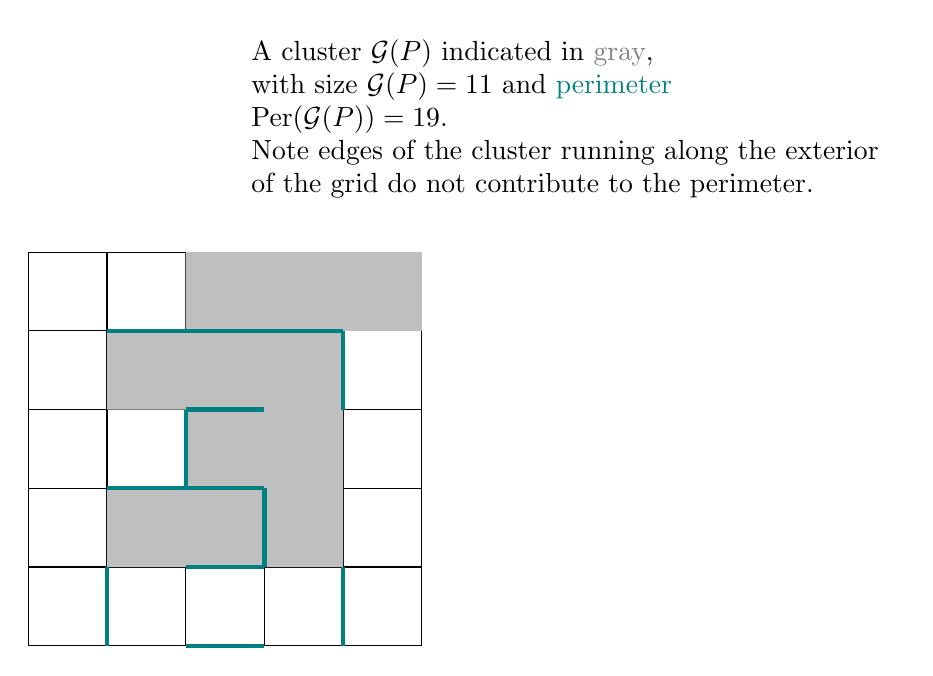
\begin{tikzpicture}[scale=1.0]

% Define grid parameters
\def\cellsize{1.0} % Size of each cell
\def\gridsize{5}   % Size of the grid (5x5)

% Draw the grid
\draw[black] (0,0) grid (\gridsize,\gridsize);

% Define the cluster cells (gray fill)
\fill[gray!50] 
    (1,1) rectangle ++(1,1) % Cell (1,1)
    (2,1) rectangle ++(1,1) % Cell (2,1)
    (3,1) rectangle ++(1,1) % Cell (3,1)
    (2,2) rectangle ++(1,1) % Cell (2,2)
    (3,2) rectangle ++(1,1) % Cell (3,2)
    (1,3) rectangle ++(1,1) % Cell (1,3)
    (2,3) rectangle ++(1,1) % Cell (2,3)
    (3,3) rectangle ++(1,1) % Cell (3,3)
    (2,4) rectangle ++(1,1) % Cell (2,4)
    (3,4) rectangle ++(1,1) % Cell (3,4)
    (4,4) rectangle ++(1,1); % Cell (4,4)

% Draw the perimeter edges (teal lines)
\draw[teal, line width=1.5pt]
    % Horizontal edges
    (1,\gridsize-1) -- (\gridsize-1,\gridsize-1) % Top row
    (2,\gridsize-2) -- (3,\gridsize-2)           % Second row
    (1,\gridsize-3) -- (3,\gridsize-3)           % Third row
    (2,\gridsize-4) -- (3,\gridsize-4)           % Fourth row
    (2,\gridsize-5) -- (3,\gridsize-5)           % Bottom row
    % Vertical edges
    (\gridsize-1,\gridsize-1) -- (\gridsize-1,\gridsize-2) % Rightmost column
    (2,\gridsize-2) -- (2,\gridsize-3)           % Second column
    (3,\gridsize-3) -- (3,\gridsize-4)           % Third column
    (1,\gridsize-4) -- (1,\gridsize-5)           % Fourth column
    (4,\gridsize-4) -- (4,\gridsize-5);          % Fifth column

% Add annotations
\node[above right, black] at (0.5*\gridsize, \gridsize+0.5) {
    \begin{tabular}{l}
        A cluster $\mathcal{G}(P)$ indicated in \textcolor{gray}{gray}, \\
        with size $\abs{\mathcal{G}(P)} = 11$ and \textcolor{teal}{perimeter} \\
        $\mathrm{Per}(\mathcal{G}(P)) = 19$. \\
        Note edges of the cluster running along the exterior \\
        of the grid do not contribute to the perimeter.
    \end{tabular}
};

\end{tikzpicture}
\end{document}